\chapter{基于库所变迁时延网的蚁群算法研究}
第二章介绍了一系列的时间Petri网,第三章提出了一种称为TTPPN的时间网子类,
并基于TTPPN对一个实际的半导体晶圆生产系统进行了建模。

本章将基于上章建立的TTPPN模型,使用算法计算出一条变迁序列。
TTPPN发射此变迁序列,会到达一个规定好的终止标识。
在实际的半导体晶圆生产系统中,最开始,晶圆会堆放在一个腔体中。
随着加工过程的运行,晶圆会被带离初始的腔体,经过一系列的环节,最终被放入到另一个腔体中。
在TTPPN中,这些腔体可被建模为库所。
因此算法的任务即为寻找一条能将一个库所中所有托肯转移到另一个库所中的变迁序列。

另外,按上一章的变迁发射逻辑,每个变迁发射都会有一个具体的时刻,将此时刻作为一个属性存入TTPPN的标识中,称为全局时刻。
TTPPN发射变迁序列生成的最终标识的全局时刻即为此系统完成晶圆加工的总耗时,称为完工时间。
实际情况下,需要完工时间越短越好。这个值将用来衡量算法的解质量。
算法从开始到找到终止标识所消耗的时间称为程序运行时间。这个值将用来衡量算法的速度。
对于启发式算法、群体智能算法来说,时间复杂度的分析十分困难。另外程序运行时间还会受操作系统进程调度策略的影响,未必能如实反映算法速度。
因此本章将记录Petri网的发射次数,用以作为分析算法速度的补充数据。
当Petri网的库所、变迁数确定时,发射变迁产生新标识的时间开销也是确定的。
而对于蚁群算法,其大部分时间开销是发射变迁带来的,因此用发射次数来表征算法的速度。
\section{基于TTPPN的基本蚁群算法}
蚁群算法(Ant Clony Optimization, ACO)是一种群智能算法,
它是由一群无智能或有轻微智能的个体(Agent)通过相互协作而表现出智能行为,
从而为求解复杂问题提供了一个新的可能性。
蚁群算法最早是由意大利学者Colorni A., Dorigo M. 等于1991年提出。
算法运行时蚂蚁会以更高的概率选择信息素浓度高的路,
而蚂蚁会为长度短的路留下更多的信息素。
因此选路机制与信息素添加机制构成了一个正反馈的逻辑,
随着程序的持续运行,正反馈会将解往更优的方向引导\cite{blum2003metaheuristics}\cite{li2015survey}\cite{colorni1992distributed}\cite{kennedy1995particle}\cite{dorigo2004ant}。

TTPPN为时间网,其托肯和变迁上均有时钟,
如果要完整的表示TTPPN,需要记录每一个托肯和变迁上的时钟。
即便两标识中所有库所中的托肯数都相同,但只要托肯上的时钟计时不同,
依然要视为不同的标识。
因此TTPPN与其不加时间的网相比,可达图会异常庞大。

但是在蚁群算法中,即便不存储TTPPN的完整信息,依然可以保证上述正反馈逻辑。
当区分标识仅考虑标识的库所向量时,可达图便可看作是一个边上权值可变的有向图。
\begin{figure}[H]
	\centering
	% Requires \usepackage{graphicx}
	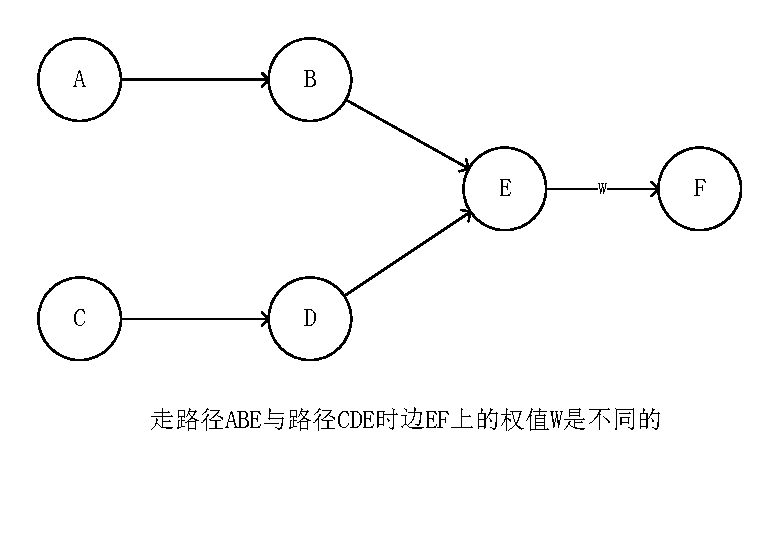
\includegraphics[scale=0.7,angle=0]{figures/可变权值图.pdf}\\
	\caption{可变权值图}
\end{figure}
边上权值会受到初始标识到此标识路径的影响。
选路机制与信息素添加机制构成的正反馈逻辑并不会被破坏,
因此即便不区分时钟计时不同的标识,依然可以使用蚁群算法。

基于TTPPN的基本蚁群算法可分为三个阶段:蚂蚁循迹阶段、信息素稀释阶段和信息素添加阶段。

\begin{algorithm}[H]
    \caption{基于TTPPN的基本蚁群算法}
    \hspace*{0.02in} {\bf 输入:} 
    变迁库所时间网$TTPPN$,变迁库所时间网的初始标识$initMarking$,蚂蚁只数$antCount$,算法迭代轮数$round$\\
    \hspace*{0.02in} {\bf 输出:}
	变迁序列$trans$
    \begin{algorithmic}[1]
		\For {$i \leftarrow 1, round$}
			\State $Ants \leftarrow$初始化$antCount$只蚂蚁放入蚂蚁集合
			\State $RG \leftarrow$初始化一个空的可达图
			\State $antsTravel(Ants,RG,TTPPN,initMarking)$ //蚂蚁循迹阶段
			\State $dilute(RG)$ //信息素稀释阶段
			\State $putPheromone(RG,Ants)$ //信息素添加阶段
		\EndFor
		\State 返回找到的最优变迁序列$trans$
    \end{algorithmic}
\end{algorithm}

蚂蚁循迹阶段是算法的主要流程,本阶段中每只蚂蚁都会独立地在可达图中进行搜索。

\begin{algorithm}[H]
	\caption{蚂蚁循迹阶段}
	\label{alg4-2}
	\begin{algorithmic}
		\Procedure {antsTravel}{$Ants$,$RG$,$TTPPN$,$initMarking$}
		\ForAll{$ant \in Ants$} //$Ants$为蚂蚁的集合
			\State $antTravel(ant,RG,TTPPN,initMarking)$ //单只蚂蚁循迹
		\EndFor
		\EndProcedure
	\end{algorithmic}
\end{algorithm}

每只蚂蚁都有一个禁忌表,蚂蚁每次会选择发射一个变迁,并把发射变迁生成的标识存入此禁忌表中,之后的搜索过程会禁止发射到禁忌表中已经有的标识,
避免蚂蚁走重复的路。
此蚂蚁共有两种结局:1、蚂蚁走到终点标识;2、蚂蚁无路可走。

\begin{algorithm}[H]
	\caption{单只蚂蚁循迹}
	\label{alg4-3}
	\begin{algorithmic}
		\Procedure {antTravel}{$ant$,$RG$}
		\State $tabu \leftarrow$ 初始化蚁群禁忌表
		\State $log \leftarrow$ 初始化蚂蚁日志
		\While {蚂蚁未到达终点并且未走到死路} 
			\State $next(ant,RG,TTPPN,initMarking,tabu,log)$ //为蚂蚁选择变迁并发射的逻辑
		\EndWhile
		\EndProcedure
	\end{algorithmic}
\end{algorithm}

蚂蚁无路可走既可能是因为蚂蚁走上了死锁标识,没有使能变迁可以发射,也可能是此标识的所有使能变迁发射后的标识均在禁忌表中出现过了。
蚂蚁会一直搜索下去直到走到终点,蚂蚁在搜索过程中会记录发射的变迁序列,用以更新可达图上的信息素和输出最后的解。
因为每只蚂蚁的搜索过程相互独立,所以每只蚂蚁搜索过程可由独立的线程并发执行,以提升效率。
蚁群算法的可达图是不带有时间信息的,仅由标识与标识通过使能变迁连接,标识为图的节点,变迁为图的有向弧。
变迁上有一个权值,称为信息素浓度,蚂蚁会根据信息素浓度,并综合考虑到禁忌表,随机选择一个使能变迁发射。
如果蚂蚁到达的标识之前未被添加进可达图,则默认这个标识的所有使能变迁上的信息素浓度是相同的。

\begin{algorithm}[H]
	\caption{蚂蚁选择变迁并发射的逻辑}
	\label{alg4-4}
	\begin{algorithmic}
		\Procedure {next}{$Ants$,$RG$,$TTPPN$,$initMarking$,$ant$,$RG$}
		\State $t=chose(RG,initMarking)$
		\State $initMarking=lanuch(TTPPN,initMarking,t)$
		\State 将当前标识添加进禁忌表$tabu$中
		\State 将发射的变迁$t$记录在蚂蚁日志$log$中
		\EndProcedure
	\end{algorithmic}
\end{algorithm}

\textbf{定义4.1}\textbf{:}
记$P_{Mt}$为可达图中标识$M$的变迁$t$上的信息素浓度,$P_{Mt}\in \mathbb{R}$。
处于标识$M$的蚂蚁选择发射变迁$t$的概率为
$
	\frac{P_{Mt}}{\sum_{i \in T} P_{Mi} }
$。
蚂蚁随机选择变迁发射的算法为轮盘赌算法。
如果有n个待选择的元素,此算法会生成n个彼此相邻的区间,区间的长度与此元素被选择的概率成正比。
算法会随机生成一个大于0,小于区间长度的数值。
这个数值落在哪个区间内,算法就会选择哪个数。

\begin{algorithm}[H]
	\caption{蚁群算法中的轮盘赌算法}
	\label{alg4-5}
	\begin{algorithmic}
		\Procedure {chose}{$RG$,$initMarking$}
		\State $total \leftarrow 0$
		\State $probability \leftarrow $ 用于存储变迁和变迁上信息素浓度的键值对集合
		\State 
		\ForAll{$t \in T$}
			\If{$t^{-} \le m$}
				\State $next \leftarrow lanuch(TTPPN,initMarking,t)$
				\If{$next \in tabu$}
					\State continue
				\EndIf
				\State $value \leftarrow$ 变迁$t$上的信息素浓度
				\State $total=total+value$
				\State $put(probability,t,value)$ //$put(probability,t,value)$指在键值对集合probability中添加键值对$(t,value)$
			\EndIf
		\EndFor
		\State $random \leftarrow $随机生成一个大于0,小于$total$的数
		\State $total=0$
		\ForAll{$t \in keys(probability)$} //$keys(probability)$表示键值对集合$probability$中键的集合
			\State $value \leftarrow get(probability,t)$ //$get(probability,t)$表示从键值对集合$probability$中取键$t$的值
			\State $total=total+value$
			\If{$total \ge random$}
				\State return true
			\EndIf
		\EndFor
		\EndProcedure
	\end{algorithmic}
\end{algorithm}

蚂蚁会根据可达图变迁上的信息素浓度的大小,随机选择一个变迁发射,并在走到终点后,为可达图增加信息素。
随着蚁群算法不断运行下去,可达图中的信息素浓度会越来越高,导致之后蚂蚁添加的信息素占总信息素浓度的比重越来越低。
在这种情况下,后期蚂蚁对解的影响将会减少。
而前期可达图中信息素尚少,蚂蚁循迹几乎是随机的,所以后期的蚂蚁比前期的蚂蚁更为重要。
因此应该加入信息素稀释机制。

\textbf{定义4.2}\textbf{:}
记$\alpha $为信息素稀释率,$\alpha \in \mathbb{R}$,$P_{Mt}^{i}$为蚁群算法第$i$轮中$P_{Mt}$的值。
记$A_{Mt}^{ji}$为第$j$只蚂蚁第$i$轮要在标识$m$上添加的信息素浓度。
$P_{Mt}^{i+1}=\alpha P_{Mt}^{i}+A_{Mt}^{ji}$

每轮可达图上的信息素都会按比例被稀释掉。
\begin{algorithm}[H]
	\caption{信息素稀释阶段}
	\label{alg4-6}
	\begin{algorithmic}
		\Procedure {dilute}{$RG$}
			\ForAll{$M \in RG$}
				\ForAll{$t \in T$}
					\State $P_{Mt}=\alpha P_{Mt}$
				\EndFor
			\EndFor
		\EndProcedure
	\end{algorithmic}
\end{algorithm}

蚁群在循迹过程中,会将到达终点标识的变迁标识序列保存起来,称为蚂蚁日志(log),并在添加信息素阶段根据蚂蚁日志,更新信息素。
如果蚂蚁日志中的标识已经在可达图中存在,则直接更新其上的信息素。
如果此标识之前从未被放入可达图,则在此时放入可达图。
因此蚁群算法的可达图是随着算法运行,逐渐扩展出来的,并不需要一开始就提供。
信息素的添加量要和路径长度成反比,在我们时间网的场景下,蚂蚁日志中的变迁标识序列中最后一个标识记录的时刻是完成调度的总耗时。
因此信息素的添加量应与这一时刻成反比。

\textbf{定义4.3}\textbf{:}
记$T_{ji}$为第$j$只蚂蚁第$i$日志的变迁标识序列中最后一个标识记录的时刻,此蚂蚁要在标识$m$上添加的信息素浓度$A_{Mt}^{ji}=\frac{C}{T_{ji}} $。

\begin{algorithm}[H]
	\caption{信息素添加阶段}
	\label{alg4-7}
	\begin{algorithmic}
		\Procedure {putPheromone}{$RG$,$Ants$}
			\ForAll{$ant \in Ants$}
				\ForAll{$M \in Markings(log)$} \\$Markings(log)$为蚂蚁日志log中的标识序列
					\If{$M \in RG$}
						\State $P_{Mt}=A_{Mt}$
					\Else
						\State 将$M$放入$RG$中
						\State $value \leftarrow 默认值$
						\State $P_{Mt}=value$
					\EndIf
				\EndFor
			\EndFor
		\EndProcedure
	\end{algorithmic}
\end{algorithm}
上述流程如果以单只蚂蚁为粒度,进行并发计算,无线程安全问题容易解决。
因为每只蚂蚁所需要的资源仅有两种:可达图、蚂蚁日志。
其中日志为每只蚂蚁私有资源,其他蚂蚁无权操作,因此无线程冲突。
而蚂蚁对于可达图有两种操作:读、写。
写操作只发生在稀释和更新信息素阶段。
而读操作发生在蚂蚁循迹阶段。
读写操作是分离的。
因此读操作不存在线程冲突。

对于写操作,有线程安全问题,因此需要加锁,并发度不如其他流程。
但通过合理选择可达图的数据结构,可以尽可能提升并发度。

\section{蚁群可达图使用的数据结构}
蚂蚁在循迹阶段,需从可达图上得出当前标识上各个使能变迁的信息素浓度。
因此蚂蚁对可达图有查询操作。

在信息素浓度稀释阶段,可达图上各个变迁的信息素浓度需按比例稀释。
因此可达图需支持修改数据的操作。

在添加信息素阶段,蚂蚁有可能探索到从未被发现的标识。
需要将这个标识的信息加入可达图中。
因此蚂蚁对可达图有添加信息的操作。

随着算法的一轮轮迭代,某些标识上的使能变迁的信息素已经被稀释到很低了。
蚂蚁走上此标识的概率极小,即便走上了,其使能变迁上信息素浓度也近乎均匀。
因此应该从可达图中删除这类标识,以节约内存。

基于以上的分析,蚁群算法的可达图需支持增、删、改、查四种操作。
所以应该选择增、删、改、查复杂度均为$O(1)$的哈希表作为数据结构实现。

可达图在算法流程中需写入数据,此操作有线程安全问题,因此需要对其加锁。
一下两种为哈希表的常规加锁方式。
\subsection{对操作方法加锁}
当算法中有线程要对可达图进行写入操作时,
需尝试取得写入操作的锁,
并在写入完成后释放锁。
锁的数量只有一个。
对于取得锁和释放锁的逻辑,均调用操作系统自带的原语以保证原子性。
如果某流程具有原子性,则此流程只有两种状态:未开始状态、已完成状态。
因此可以使用CAS原语实现加锁。
CAS的功能是将某地址的值与给定值比较并交换,并根据比较结果返回特定值。
CAS方法具有原子性,利用CAS方法的特点可以设计互斥锁。
互斥锁实现方法如下:

1、判断CAS操作是否成功,如果不是则重复此步;

2、执行写可达图的操作;

3、使用CAS将特定地址的值置回初值。


使用此逻辑,保证了不可能有两个线程同时修改可达图,从根本上解决了线程安全问题。
但是这种加锁逻辑,过于粗糙,大大降低了并发度。

使用CAS锁,如果某线程未取得锁,它会一直尝试取得锁。
可以使用信号量机制,直接让处理机暂停执行此线程,从而执行其他线程,来提高效率。
\subsection{对数据加锁}
即便是对可达图进行修改,如果修改的不是同一个标识的数据,也是不会有线程安全问题的。
而同时对同一个标识进行写操作,完全是小概率事件。
所以对具体标识进行加锁是更为高效的选择。

基于哈希表的底层原理,实际上是对哈希表内部数组的各个地址进行加锁,锁的数量最多为内部数组长度。
当写操作需要处理某地址的数据,先尝试取得此地址上的锁,并在写入完成后释放锁。

锁的数量增加会带来额外的内存开销。
如果需减少这部分的内存开销可以将锁加在地址的区间上,以减少锁的数量。
\section{备份可达图提高算法并发度}
本算法分为三个阶段:蚂蚁循迹阶段、信息素稀释阶段、信息素添加阶段。
原算法中三阶段是串行的。
蚂蚁需要先循迹,得到解后才能添加信息素,因此第一阶段和第三阶段存在依赖关系,必然是串行的。
然而第二阶段和一、三阶段的依赖关系并不明确。
理论上第二阶段和第三阶段可看作是一个大阶段,
即更新信息素阶段。
而第一阶段和第三阶段本质上并没有依赖关系,
只因为第一阶段蚂蚁循迹需要读可达图,第二阶段可达图稀释需要写可达图,
因此为保证线程安全,将其分为两个阶段。

如果将可达图备份一份,这两个阶段是可以并发执行的。

现将可达图分为两份,主可达图($RG$)与副可达图($RGCopy$)。
这两份可达图互为副本,在之后蚁群算法一轮轮迭代中会交替充当主可达图供蚁群使用。

在蚂蚁循迹阶段另外加入一个线程,专门用于完成可达图备份与稀释。

主可达图因为上一轮被修改了信息,这部分信息未被加入副可达图中,
副可达图也需要同步这部分修改。

修改的内容分为三部分:对原标识的信息素更新、添加新标识、删除信息素浓度过低的标识。
因此需遍历原可达图,并基于此修改副可达图的信息。
再遍历副可达图,删除原可达图中不存在的标识。

完成蚂蚁循迹流程后,交换原副可达图。

\begin{algorithm}[H]
	\caption{备份可达图}
	\label{alg4-9}
	\begin{algorithmic}
		\Procedure {copy}{$RG$,$RGCopy$}
			\ForAll{$m\in RG$}
				\If{$m \in RGCopy$}
					\State 同步$m$上的信息素浓度
				\Else
					\State 将$m$添加入$RGCopy$中
				\EndIf
			\EndFor
				\ForAll{$m \notin  RGCopy$}
				\If{$m \in RG$}
					\State 从$RGCopy$中删除$m$
				\EndIf
			\EndFor
		\EndProcedure
	\end{algorithmic}
\end{algorithm}

\section{蚁群求解实际问题}
本节将使用蚁群算法求解第四章对实际晶圆生成系统建立的模型。
为衡量蚁群算法解的质量,需要知道模型的最优调度策略。
本节将使用迪杰斯特拉算法求解Petri网模型的最优变迁序列。
\subsection{基于迪杰斯特拉算法求解Petri网最优变迁序列}
迪杰斯特拉算法用于求取图的最短路径。
如果图的节点数为n,此算法可以在$O(nlog(n))$的时间复杂度下得出各节点到起点的最短路径。

基于时间网的背景,设计迪杰斯特拉算法。

\subsubsection{存放将要扩展的标识的集合}
设计一个集合,此集合专门用于存放接下来将要扩展的标识,命名为$OPEN$集合。
Petri网的可达图是随算法运行动态添加进内存中的,所以$OPEN$中一开始只有初始标识,
随着程序的运行,如果遇到有扩展价值的标识,此标识会被放入$OPEN$中。

$OPEN$会被取出标识进行扩展,也会被放入标识。
但基于迪杰斯特拉算法的机制,取出的标识应该是集合中离原点最近的标识,
也就是全局时间最短的标识。

如果遍历这个集合寻找全局时间最短的标识,当集合大小为$n$时,其时间复杂度为$O(n)$。
但是如果使用小根堆去实现,其时间复杂度为$O(log(n))$。
因此本算法将使用小根堆作为此集合的实现。

\subsubsection{已经扩展的标识的集合}
此集合专门用于存放已经扩展的标识,命名为$CLOSE$集合。
当一个标识从$OPEN$取出,并且它的所有变迁均被处理过,就会放入此集合中。
因为每次处理的标识都是$OPEN$中全局时间最短的标识,
所以当此标识进入$CLOSE$中,如果之后再扩展到它,如果时间网可达图路径上的时间间隔是确定的,其全局时间必然更长。
所以当标识已经在$CLOSE$中了,是没有扩展的意义的。

但实际上时间网可达图路径上的权值是可变的,所以$CLOSE$表中存储的为键值对,键为标识,值为目前到达此标识的最短时间。
此后判断标识是否值得扩展,应该判断到达此标识的全局时间是否比$CLOSE$表中记录的最短时间短,
如果此时间确实更短,才去扩展此标识。

$CLOSE$涉及到两种操作:将已完成扩展的标识存入此集合中、查询标识是否在此集合中。
因此本算法选取哈希表作为此集合的数据结构实现。哈希表存与查的时间复杂度均为$O(1)$。
使用哈希表实现的$CLOSE$其底层是一个固定长度的数组。
标识需要得到$CLOSE$底层数组的一个元素索引,才能进入$CLOSE$表。
进入$CLOSE$表的标识会被存放在特定索引上。
此索引是根据哈希值得出的,哈希值是使用哈希函数得出的,哈希函数的输入是标识向量。
对于哈希值相同的标识,本$CLOSE$表会将其统一存放在一棵红黑树中。
如果红黑树的节点数为$n$,其增删改查的时间复杂度是$log(n)$。

\subsection{算法流程}
迪杰斯特拉算法每次会从$CLOSE$中取一个全局时间最短的标识$curr$,如果此标识就是终点标识,则找到终点。
如果$CLOSE$集合取空都未找到终点,则说明终点不可达。
对$curr$的所有使能变迁均发射一次,如果发射产生的新标识$next$已经在$OPEN$中存在,并且其全局时间更短,则将其取出,更新其全局时间后再放入。
在$OPEN$中查询标识的时间复杂度为$O(log(n))$,往其放入标识的时间复杂度为$O(log(n))$。
如果$next$的全局时间已经高于$CLOSE$中对于标识处记录的最短时间,则没有必要扩展此标识,如果不存在,之前查找时也没在$OPEN$中找到就将此标识放入$OPEN$中。
当$curr$的所有使能变迁均处理完成,将其放入$CLOSE$中。

迪杰斯特拉算法流程如下所示:

\begin{algorithm}[H]
    \caption{基于时间网的迪杰斯特拉算法}
    \hspace*{0.02in} {\bf 输入:} 
    变迁库所时间网$TTPPN$,变迁库所时间网的初始标识$initMarking$,终点标识$endMarking$\\
    \hspace*{0.02in} {\bf 输出:}
	变迁序列$trans$
    \begin{algorithmic}[1]
		\For {$i \leftarrow 1, round$}
			\State 往$OPEN$放入初始标识$initMarking$
			\While{$OPEN$不为空}
				\State $curr \leftarrow$从$OPEN$中取出全局时间最小的标识
				\ForAll{$t\in curr$的使能变迁}
					\State $next \leftarrow launch(TTPPN,curr,t)$
					\If{$next$在$OPEN$中且全局时间更短}
						\State 更新$OPEN$中$next$的全局时间
					\EndIf
					\If{$next$值得扩展}
					\State 将$next$放入$OPEN$
					\EndIf
				\EndFor
				\State 将$curr$放入$CLOSE$中
			\EndWhile
		\EndFor
		\State 返回找到的最优变迁序列$trans$
    \end{algorithmic}
\end{algorithm}

\subsection{实验和结果分析}
在处理器为i5-1130G7,最大内存为8GB的设备上,排除文件读入、结果输出的耗时,仅在调用算法前后记录系统时间戳,
分别使用迪杰斯特拉算法和蚁群算法求解第五章建立的晶圆制造系统的模型。

\subsubsection{迪杰斯特拉算法的实验结果分析}
以下是使用6GB内存,迪杰斯特拉算法的结果。

变迁序列为:$t_{1}$->$t_{7}$->$t_{1}$->$t_{2}$->$t_{1}$->$t_{17}$->$t_{3}$->$t_{7}$->$t_{16}$->$t_{1}$->$t_{23}$->$t_{2}$->$t_{1}$->$t_{17}$->
$t_{27}$->$t_{7}$->$t_{16}$->	$t_{1}$->$t_{2}$->$t_{1}$->$t_{4}$->$t_{14}$->$t_{24}$->$t_{12}$->$t_{22}$->$t_{1}$->
$t_{13}$->$t_{29}$->$t_{11}$->$t_{22}$->$t_{1}$->$t_{14}$->$t_{12}$->$t_{22}$->$t_{20}$->$t_{18}$->$t_{1}$->$t_{4}$->$t_{14}$->
$t_{24}$->$t_{12}$->$t_{22}$->$t_{20}$->$t_{18}$->$t_{13}$->$t_{1}$->$t_{29}$->$t_{11}$->$t_{22}$->$t_{20}$->$t_{18}$->$t_{14}$->
$t_{1}$->$t_{12}$->$t_{22}$->$t_{20}$->$t_{18}$->$t_{1}$->$t_{4}$->$t_{14}$->$t_{24}$->$t_{12}$->$t_{22}$->$t_{20}$->$t_{18}$->
$t_{13}$->$t_{20}$->$t_{18}$->$t_{8}$->$t_{29}$->$t_{22}$->$t_{14}$->$t_{20}$->$t_{18}$->$t_{9}$->$t_{22}$->$t_{20}$->$t_{18}$->
$t_{20}$->$t_{18}$->$t_{4}$->$t_{10}$->$t_{9}$->$t_{24}$->$t_{22}$->$t_{6}$->$t_{8}$->$t_{22}$->$t_{28}$->$t_{10}$->$t_{20}$->
$t_{18}$->$t_{9}$->$t_{22}$->$t_{20}$->$t_{18}$->$t_{20}$->$t_{18}$->$t_{4}$->$t_{10}$->$t_{9}$->$t_{22}$->$t_{20}$->$t_{18}$

完工时间为:1600.8s

程序运行时间为:8.972s

迪杰斯特拉算法每次都会选取离起点最近的节点进行扩展,因此扩展过程为一层层推进,其扩展过的可达标识数与可达图成比例。
本算法在使用变迁发射方法$launch$时会使用到标识的时钟信息,
而时间网的标识数巨大,为节约内存开销,本算法仅将标识向量存入$CLOSE$中。
因此在扩展过程中会产生大量的垃圾信息,需要被垃圾回收。
内存大小影响垃圾回收的次数,内存越大,垃圾回收次数越少。

分别测试从1GB内存到6GB内存迪杰斯特拉算法的程序运行时间。

\begin{table}[H]
	\centering
	\caption{内存与程序运行时间关系}
	\resizebox{!}{!}{
		\begin{tabular}{l|lllllllll}
			\toprule
			内存(GB) & 1 & 2 & 3 & 4 & 5 & 6 \\ \hline
			程序运行时间(s) & 12.695 & 10.930 & 9.031 & 8.752 & 8.803 & 8.972 \\
			\bottomrule
		\end{tabular}
	}
\end{table}

\begin{figure}[H]
	\centering
	% Requires \usepackage{graphicx}
	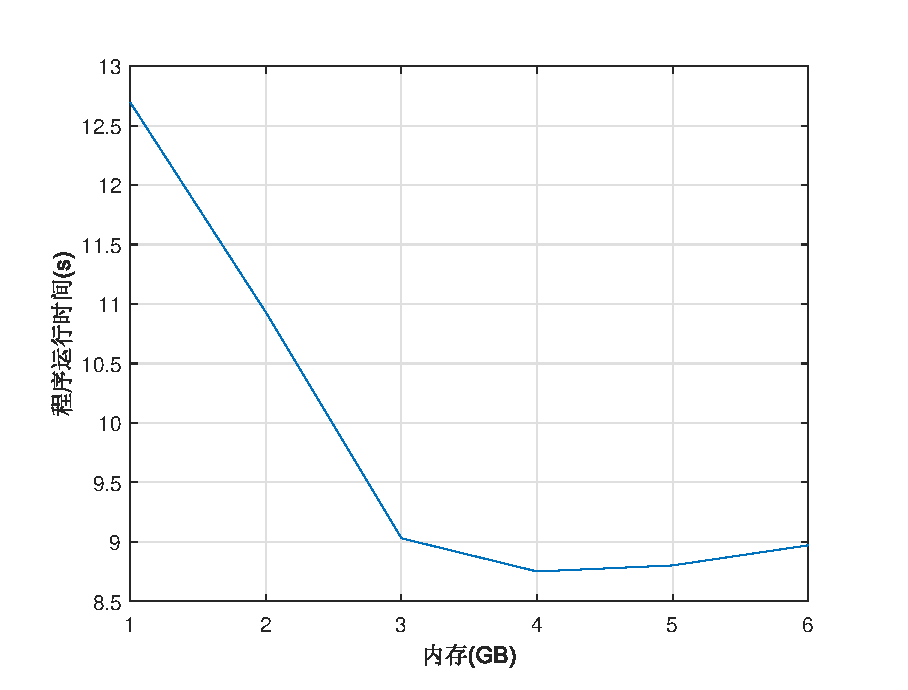
\includegraphics[scale=1.00,angle=0]{figures/mem_t.eps}\\
	\caption{迪杰斯特拉算法内存与程序运行时间关系}
\end{figure}

如上图所示,随着内存的增加,程序运行时间有下降的趋势,当内存增加到3GB时,程序运行时间稳定在9s左右。

\subsubsection{蚁群算法的实验结果分析}
以下是使用6GB内存,蚁群算法100只蚂蚁迭代100轮的结果。

变迁序列:$t_{1}$->$t_{2}$->$t_{1}$->$t_{7}$->$t_{17}$->$t_{3}$->$t_{16}$->$t_{23}$->$t_{1}$->$t_{2}$->$t_{1}$->$t_{4}$->$t_{13}$->$t_{24}$->$t_{7}$->$t_{14}$->$t_{3}$->$t_{4}$->$t_{9}$->$t_{10}$->$t_{24}$->$t_{22}$->$t_{1}$->$t_{11}$->$t_{13}$->$t_{23}$->$t_{21}$->$t_{19}$->$t_{12}$->$t_{21}$->$t_{18}$->$t_{17}$->$t_{20}$->$t_{18}$->$t_{1}$->$t_{27}$->$t_{24}$->$t_{10}$->$t_{28}$->$t_{12}$->$t_{14}$->$t_{23}$->$t_{22}$->$t_{8}$->$t_{21}$->$t_{24}$->$t_{6}$->$t_{19}$->$t_{12}$->$t_{22}$->$t_{17}$->$t_{8}$->$t_{27}$->$t_{22}$->$t_{1}$->$t_{7}$->$t_{1}$->$t_{17}$->$t_{7}$->$t_{20}$->$t_{18}$->$t_{23}$->$t_{1}$->$t_{2}$->$t_{1}$->$t_{17}$->$t_{7}$->$t_{20}$->$t_{19}$->$t_{3}$->$t_{28}$->$t_{14}$->$t_{27}$->$t_{12}$->$t_{21}$->$t_{16}$->$t_{18}$->$t_{24}$->$t_{14}$->$t_{4}$->$t_{9}$->$t_{21}$->$t_{18}$->$t_{6}$->$t_{28}$->$t_{8}$->$t_{6}$->$t_{24}$->$t_{10}$->$t_{22}$->$t_{4}$->$t_{9}$->$t_{10}$->$t_{21}$->$t_{18}$->$t_{9}$->$t_{22}$->$t_{20}$->$t_{18}$->$t_{8}$->$t_{21}$->$t_{18}$->$t_{20}$->$t_{18}$->$t_{20}$->$t_{18}$

完工时间:2554.7s

程序运行时间:23.374s

此结果无论是完工时间还是程序运行时间,均要长于迪杰斯特拉算法的解。

导致此结果的可能原因有3个:算法不能收敛、算法收敛到较差解、算法收敛慢。

基于以上的分析,设计实验。
依次提高迭代轮数,观察完工时间,如果随迭代轮数增加,完工时间分布随机,则说明算法未收敛。
如果随迭代轮数增加,完工时间区域稳定值,并且稳定值接近迪杰斯特拉算法的解,说明算法收敛慢,如果稳定值显著高于迪杰斯特拉的解,
说明算法收敛到较差解。

另外,在计算机CPU有限的情况下,提高蚂蚁只数会时程序频繁进行线程切换,增大程序运行时间。
使用需要探寻蚂蚁只数与算法效率的关系。

将迭代轮数从10轮每次递增10轮直到100轮,统计完工时间,观察蚁群算法是否有收敛趋势。

\begin{table}[H]
	\centering
	\caption{蚁群算法迭代轮数与完工时间的关系}
	\resizebox{\linewidth}{!}{
		\begin{tabular}{l|lllllllllllll}
			\toprule
				轮数 & 10 & 20 & 30 & 40 & 50 & 60 & 70 & 80 & 90 & 100 \\ 
				\hline
				完工时间(s) & 2554.7 & 2254.1 & 1956.1 & 1921.7 & 2223.8 & 2494.7 & 2513.5 & 2487.9 & 2393.8 & 2554.7 \\
				\bottomrule
			\end{tabular}
	}
\end{table}

如图所示,蚁群算法在本场景下并没有收敛,迭代轮数在30轮之前,完工时间有下降趋势,但随着轮数的增加,完工时间也增加,最终有稳定在2500.0s的趋势。

从这个结果可以看出,此蚁群算法收敛到一个较差的解上,而且并不是收敛到局部最优解,因为随着迭代轮数增加,算法曾到达了较优的解,但依然有向差解接近的趋势。

为证明前30轮确实有下降趋势,而非是偶然现象,将迭代轮数从1轮每次递增10轮直到10轮,统计完工时间。

\begin{table}[H]
	\centering
	\caption{蚁群算法迭代轮数与完工时间的关系(小轮数)}
	\resizebox{\linewidth}{!}{
		\begin{tabular}{l|lllllllllllll}
			\toprule
			轮数 & 1 & 2 & 3 & 4 & 5 & 6 & 7 & 8 & 9 & 10 \\ \hline
			完工时间(s) & 3274.6 & 3136.1 & 3153.8 & 3024.6 & 2952.2 & 2840.0 & 2708.3 & 2630.0 & 2600.5 & 2554.7 \\
			\bottomrule
		\end{tabular}
	}
\end{table}

\begin{figure}[H]
	\centering
	% Requires \usepackage{graphicx}
	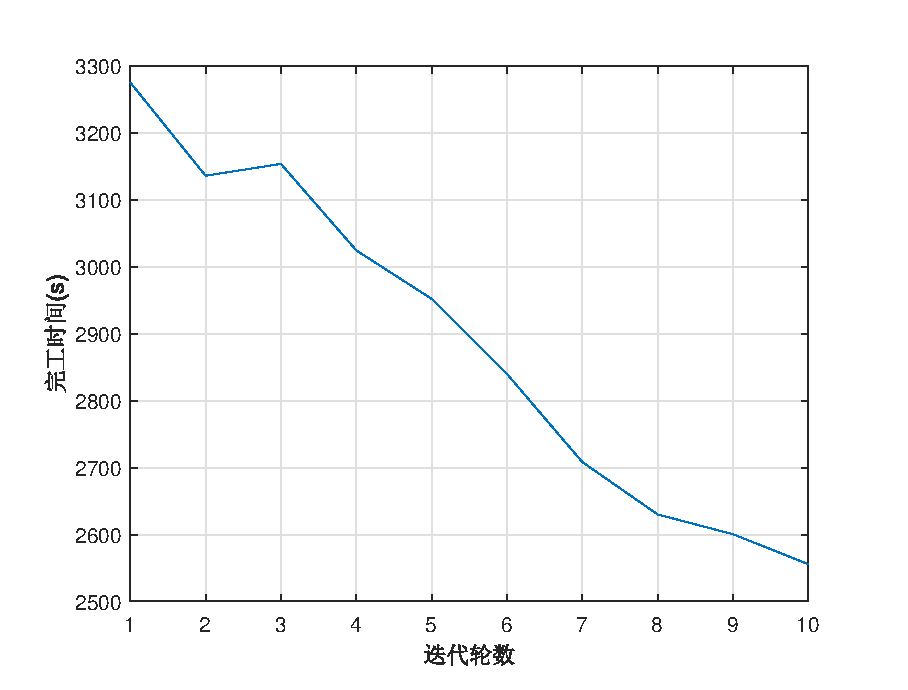
\includegraphics[scale=1.00,angle=0]{figures/round_t_small.eps}\\
	\caption{蚁群算法迭代轮数与完工时间关系(1到10轮)}
\end{figure}

如上图所示,低轮数时蚁群算法确实有收敛趋势。

本程序中每只蚂蚁都是一个线程,如果线程数量小于CPU数量,各个线程能并行指向,彼此互不影响。
而如果线程数量高于CPU数量,CPU就需要不断第切换到不同的线程,以实现程序并发地执行。
如果两线程竞争一个CPU,必然会导致其中一个线程等待。
因此随蚂蚁只数增加,程序运行时间会增加。
此外线程切换本身也是有开销的。
所以需要探寻蚁群算法蚂蚁只数对完工时间的影响,得出一个恰当的蚂蚁只数,并以此合理配置CPU数量。

为了观察蚂蚁只数对算法收敛性的影响,固定迭代轮数为10轮,从10只蚂蚁每次递增10只直到100只对此模型进行求解,观察完工时间。

\begin{table}[H]
	\centering
	\caption{蚁群算法蚂蚁只数与完工时间的关系}
	\resizebox{\linewidth}{!}{
		\begin{tabular}{l|lllllllllllll}
			\toprule
				蚂蚁只数 & 10 & 20 & 30 & 40 & 50 & 60 & 70 & 80 & 90 & 100 \\ \hline
				完工时间(s) & 2799.9 & 2404.6 & 3184.9 & 2314.9 & 2637.2 & 2718.6 & 2599.7 & 2596.0 & 2894.7 & 2554.7 \\
			\bottomrule	
		\end{tabular}
	}
\end{table}

\begin{figure}[H]
	\centering
	% Requires \usepackage{graphicx}
	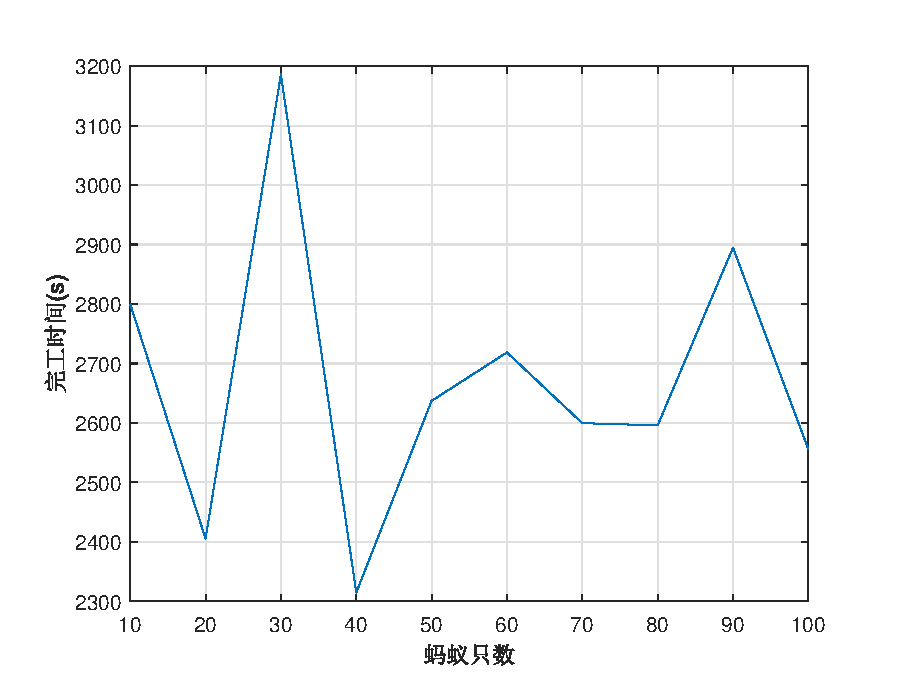
\includegraphics[scale=1.00,angle=0]{figures/count_t.eps}\\
	\caption{蚁群算法迭代轮数与完工时间关系(1到10轮)}
\end{figure}

如上图所示,随着蚂蚁只数的增加,完工时间是随机的,这意味着可能10只蚂蚁以后,蚂蚁只数就对算法收敛性影响不大了。

为表明低蚂蚁只数时,蚂蚁只数对算法收敛是有影响的,固定迭代轮数为10轮,从1只蚂蚁每次递增1只直到10只对此模型进行求解,观察完工时间。

如果蚂蚁只数在增加到一定值后,对解质量影响不大,则应该让蚁群算法运行在CPU数量高于此蚂蚁只数的机器上,
以避免线程切换与等待的开销,提升算法运行效率。

但是如果蚂蚁只数较高,应该选择处理器更多的GPU来运行蚁群算法。
本蚁群算法的可达图是动态扩展的,因此存在大量内存申请与清理的操作,此操作不适合在GPU上使用,
所以本文的代码是为CPU编写的。

\begin{table}[H]
	\centering
	\caption{蚁群算法蚂蚁只数与完工时间的关系(小只数)}
	\resizebox{\linewidth}{!}{
		\begin{tabular}{l|lllllllllllll}
			\toprule
			蚂蚁只数 & 1 & 2 & 3 & 4 & 5 & 6 & 7 & 8 & 9 & 10 \\ \hline
			完工时间(s) & 3640.5 & 3760.5 & 3262.0 & 3362.1 & 3256.0 & 3008.7 & 2651.0 & 2684.5 & 2752.9 & 2799.9 \\
			\bottomrule	
		\end{tabular}
	}
\end{table}

\begin{figure}[H]
	\centering
	% Requires \usepackage{graphicx}
	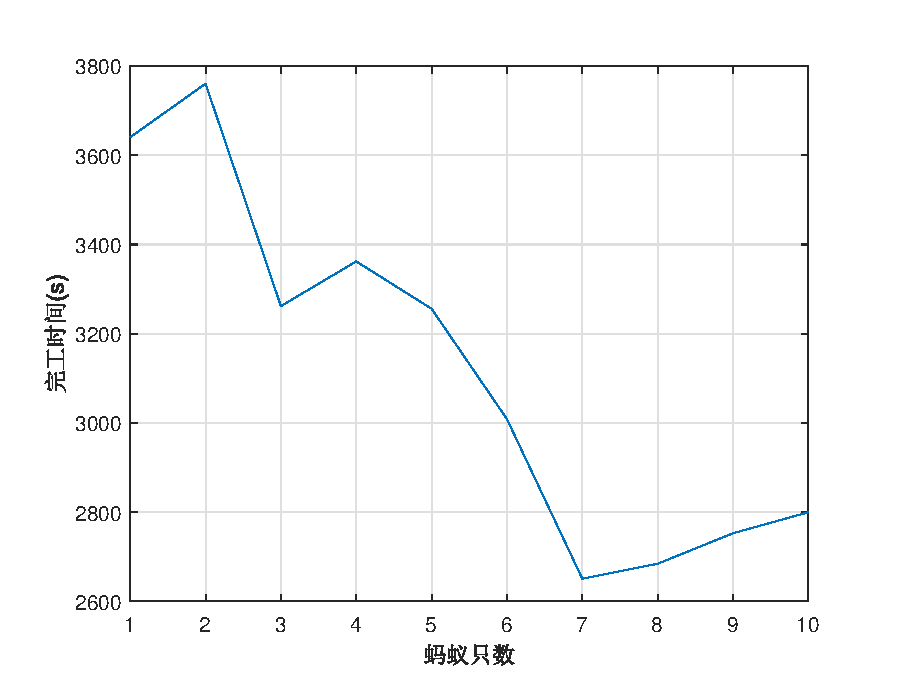
\includegraphics[scale=1.00,angle=0]{figures/count_t_small.eps}\\
	\caption{蚁群算法迭代轮数与完工时间关系(1到10轮)}
\end{figure}

如上图所示,在蚂蚁数量较少时,蚂蚁只数越大,完工时间越小。

综上,提升蚁群算法蚂蚁只数、和算法迭代次数,在一开始会对算法收敛性有较大贡献。随着蚂蚁只数增加到10只后,再增加蚂蚁只数对算法影响不大。
当迭代轮数增加到30轮以后,蚁群算法的解有恶化的趋势,再继续增加迭代轮数会使算法稳定在一个较差的解。

但是无论如何配置蚂蚁只数和迭代轮数,都无法使解向迪杰斯特拉算法求出的解靠近。下一节将继续分析蚁群算法解的情况,并且尝试了一系列优化方案。
\section{改进的蚁群算法}
基于上一小节的数据进行分析,原始的蚁群算法存在求解特定时间网的变迁序列时存在缺陷。
如果某时间Petri网的最优变迁序列上的使能变迁很少,
而完工时间较差的变迁序列彼此又互相连通,
原始蚁群算法便无法收敛。
其原因为走上最优解的蚂蚁有更高的概率走入死锁标识,失去添加信息素的资格。
而走向较差解的蚂蚁会有更高的概率走向终点标识,并在可达图上留下信息素。
原始蚁群算法的正反馈机制被打破,使算法无法收敛。
为修复这一异常,本文对原始蚁群算法进行了如下改进。
\subsection{超级蚂蚁机制}
如果此蚂蚁的解比目前的最优解还优,则赋予它添加更多信息素的权利,能添加的额外的信
息素和对解优化的贡献相关。
这么做是为了削弱之前非最优解的蚂蚁对流程的影响。当某蚂蚁运气好,得出的解远好于目
前的解,便可迅速提升这个解上的信息素,从而将误入歧途的蚂蚁重新引入正轨。

\textbf{定义4.5}\textbf{:}
记$MinTime$为蚁群算法运行时,当前得到的最短完工时间。
$CurrTime$为当前蚂蚁完成循迹后得出的完工时间。
$\beta$为此蚂蚁添加信息素的增益。
\begin{equation}
	\beta=\left\{
		\begin{aligned}
			1 \quad MinTime-CurrTime \leqslant 0\\
			MinTime-CurrTime \quad MinTime-CurrTime > 0\\
		\end{aligned}
		\right.
		\nonumber 
\end{equation}
此蚂蚁添加的信息素应乘上此增益。
因此第$j$只蚂蚁第$i$轮要在标识$m$上添加的信息素浓度$A_{Mt}^{ji}$应修改为
$$
A_{Mt}^{ji}=\beta A_{Mt}^{ji}
$$
当此蚂蚁循迹得出的解好于目前找到的最优解,它添加的信息素会被增益$\beta$放大。
当得出的解的完工时间越短,增益越大。
蚁群算法出现局部收敛时,
使用此机制,蚂蚁只要以小概率探索到了局部以外的更优解,
此解便会被添加大量信息素,
引导其他蚂蚁探索新解,
跳出局部收敛。

此蚂蚁需将找到的解更新为新的最优解。
因此在每只蚂蚁的添加信息素逻辑中需添加一段更新最优解流程。
\begin{algorithm}[H]
	\caption{更新最优解}
	\label{alg4-10}
	\begin{algorithmic}
		\Procedure {renNewMinTime}{}
			\If{$\beta>1$}
			\State $MinTime=CurrTime$
			\EndIf
		\EndProcedure
	\end{algorithmic}
\end{algorithm}

此流程中需修改$MinTime$这一全局变量。
而添加信息素逻辑是并发执行的,因此此处$MinTime$有可能同时被多个线程写入。
但因为此处即便有线程安全问题,也不影响算法执行,因此为提高并发度,不进行加锁。
\subsection{贪心选取初始信息素}
原算法蚂蚁遇到从未走过的地点(没有一只蚂蚁去过的地点),会以平均的概率选取下一步。
如果蚂蚁所在标识的各使能变迁是等价的,并不知道哪个变迁更优,蚂蚁在首次经过此标识时确实应该以平均的概率选择一条变迁。
但结合实际背景,这些变迁并不等价。
加工腔中的晶圆如果加工完毕,应该尽早取走。
基于此特点,
现将蚂蚁初次选路的策略修改为以更大的概率选择近的路。

将原算法中遇到新标识时构建新信息素对象的逻辑修改为以下逻辑。
\begin{algorithm}[H]
	\caption{贪心选取初始信息素}
	\label{alg4-11}
	\begin{algorithmic}
		\Procedure {greedyInitPheromone}{}
			\ForAll{$t\in T$}
				\If{$t^{-} \le m$}
					\State $nextMarking \leftarrow lanuch(currMarking,t)$
					\State 将变迁$t$上的信息素浓度设置为$time(nextMarking)-time(currMarking)$
					\\$time(marking)$为取得标识$marking$全局时间的方法
				\EndIf
			\EndFor
		\EndProcedure
	\end{algorithmic}
\end{algorithm}
对于此标识的所有使能变迁,均发射一次得出此标识的后继标识。
按这些后继标识的全局时间对这些变迁分配初始信息素。
时间越短初始信息素浓度越高。

这是一种贪心的思想。
发射使后继标识全局时间最短的变迁,意味着寻求单步最优的变迁发射。
实际生产系统中单步最优构成的解往往质量不差,因此这种逻辑在某些场景下,效果不错。
但如果模型最优解远离贪心解,此机制探寻新路径时依然会使用贪心的逻辑,会影响算法的收敛效率。
因此下一节将提出一种约束较弱的贪心策略。
\subsection{使用贪心算法预添加信息素}
与上一节使用的思想类似,使用贪心的思想优化算法。
具体逻辑为:
先使用贪心算法求解出一个解,在此解的变迁标识序列上添加一部分信息素。
再使用蚁群算法在此基础上继续求解。

贪心算法会不断地发射使后继标识全局时间最短的变迁,直到找到终点。
因为可达图中存在死锁标识,需为算法加入回溯机制,
遇到死锁标识时,回溯,并发射使后继标识的全局时间次大的变迁。

因此定义一个函数$find(marking)$,
此函数的功能为判断以标识$marking$为初始标识,判断是否能探索到与终点标识连通的路径。
\begin{algorithm}[H]
	\caption{贪心算法}
	\label{alg4-12}
	\begin{algorithmic}
		\Procedure {find}{$marking$}
			\If{$marking$为终点标识}
				\State return true
			\EndIf
			\State 对$marking$的使能变迁按全局时间进行排序,并装入$enableTrans$中
			\ForAll{$t \in enableTrans$}
				\State $nextMarking \leftarrow lanuch(t,currMarking)$
				\If{$nextMarking$被扩展过}
					\State continue
				\EndIf
				\If{$find(nextMarking)$}
					\State return true
				\EndIf
			\EndFor
			\State return false
		\EndProcedure
	\end{algorithmic}
\end{algorithm}
此函数使用递归实现了回溯功能。

在函数运行时一并记录发射的变迁,如果发生回溯,删除回溯的变迁,便得到一条变迁序列。
基于此序列预先为可达图分配信息素。

\subsection{复活蚂蚁}
当蚂蚁走到死锁标识时循迹结束,此时得到的变迁序列并不能到达终点标识,因此无法基于此序列添加信息素。
如果最优解附近存在大量死锁,那么大部分最优解附近的蚂蚁将失去添加信息素的资格,反而使得差解信息素浓度过高。
本节设计了一种机制,可以为使走上死锁的蚂蚁复活。

\textbf{定义4.6}\textbf{:}
记$similarity(s_{1},s_{2})$为标识序列$s_{1},s_{2}$的相似度。\\
$sameMarkingCount(s_{1},s_{2})$为标识序列$s_{1},s_{2}$中相同标识的数量。
$length(s_{1})$为$s_{1}$中标识的数量。\\
计算方法为:
$$
	similarity(s_{1},s_{2})=\frac{sameMarkingCount(s_{1},s_{2})}{length(s_{1})} 
$$

如果此蚂蚁死亡,则将其替换为活蚂蚁中与其相似度最高的蚂蚁。
\subsection{蚁群算法与模拟退火算法结合}
如果蚁群算法真的如预期,应该是会随着迭代次数的增加,收敛到一个最优解。这意味着最
优解实际上是出现在后期的。因此前期解的重要性不如后期。尽管本蚁群算法每轮都会去稀释信息素,但是是对信息素浓度总体进行成比例稀释。而信息素浓度分为两部分:初始信息
素+添加信息素。在前期解的重要性较弱的情况下,应该让蚂蚁更为随机地选择路径。所以前期应该降低添加信息素所占比例。
基于此思路,设计模拟退火机制:对添加信息素添加限制,随着轮数增加,逐步放开此限制。

\textbf{定义4.6}\textbf{:}
记$\varepsilon $为蚂蚁添加信息素的增益,
$i$为蚁群算法当前迭代轮数,
$round$为蚁群算法的总轮数。
$$
	\varepsilon=\frac{i}{round}
$$
将第$j$只蚂蚁第$i$轮要在标识$m$上添加的信息素浓度$A_{Mt}^{ji}$应修改为
$$
A_{Mt}^{ji}=\varepsilon A_{Mt}^{ji}
$$
随着轮数增加,增益$\varepsilon $会逐渐增加,加大了后期蚂蚁的重要性。

先前代码中为了加速收敛,提升了对解有贡献蚂蚁的地位。
这种蚂蚁出现在前期会让期待解变得很苛刻,以至于后期难有蚂蚁成为对解有贡献蚂蚁。
而模拟退火机制会削弱前期蚂蚁的地位。
两种机制实际上是矛盾的。

\subsection{蚂蚁回溯}
基于对本测试用例的解的分析,未避免走上最优解的蚂蚁重新走上岔路而死亡,
最为直观的策略为使蚂蚁拥有回溯的功能。
直接添加回溯功能会使蚂蚁不能死去,
以至于所有蚂蚁都要等待最后一只蚂蚁走到终点才能进行添加信息素的流程。
这无疑会极大地增加算法的时间开销。
所以应该设置蚂蚁寿命上限,
来提前结束对解优化意义不大的蚂蚁流程。
基于以上的分析,此寿命上限理应是当前最优解的全局时间。
但如果使用全局时间,
意味着其他蚂蚁依然会搜索以此全局时间为半径的部分可达图,
时间复杂度过大。
所以本算法倾向于使用最长跳数为蚂蚁寿命上限。

在原蚁群算法当蚂蚁循迹时,所有的后继标识均已在禁忌表中存在,以为着蚂蚁死亡。
在蚂蚁死亡时,将蚂蚁的当前标识替换为蚂蚁日志中倒数第二个标识,
再删除日志的最后一个标识,
便完成了回溯。

\begin{algorithm}[H]
	\caption{蚂蚁回溯}
	\label{alg4-13}
	\begin{algorithmic}
		\Procedure {antTraceBack}{}
			\State $currMarking \leftarrow log[length(log)-2]$
			\State 删除$log$中最后一个标识
		\EndProcedure
	\end{algorithmic}
\end{algorithm}

在执行回溯操作时,不能从禁忌表中删除回溯的标识。
回溯完成后,因为回溯掉的标识依然存在于禁忌表中,因此蚂蚁再次出发时,不会走向被回溯的标识。

使用蚂蚁跳数作为寿命,需要在单只蚂蚁循迹流程执行$next$方法后对此蚂蚁寿命加1。
将这种策略定义为最小步数策略(Min Step Strategy)。
\begin{algorithm}[H]
	\caption{最小步数策略}
	\label{alg16}
	\begin{algorithmic}
		\Procedure {minStepStrategy}{}
			\While{蚂蚁未到达终点且蚂蚁未到达寿命上限}
				\While{蚂蚁死亡}
					\State $antTraceBack()$
				\EndWhile
				\State $next()$
				\State 蚂蚁寿命加1
			\EndWhile
		\EndProcedure
	\end{algorithmic}
\end{algorithm}
此策略中蚂蚁寿命将由两部分组成:解的长度、蚂蚁回溯次数。

\textbf{定义4.7}\textbf{:}
记蚂蚁寿命为$life$,解的长度为$length$,蚂蚁回溯次数为$back$。
$$
	life=length+back
$$
本质上蚂蚁寿命上限的大小表示着蚂蚁的循迹能力。
寿命上限越大,循迹能力越强。
因此如果要保证最终解的质量需要较大的蚂蚁寿命上限。
而在此机制下,蚂蚁寿命上限会受到解长度的影响。
如果将解分为优解与差解,比较其长度,有两种区别的形式:
优解长差解短、差解长优解短。

当差解长优解短时,一旦寿命上限收敛到优解时,蚂蚁将失去探寻差解的能力。
这对于解质量无不良影响。
但是当情况为优解长差解短时,一旦寿命上限收敛到差解时,蚂蚁将失去探寻优解的能力。
会使解质量变差。

因此应该将解长度对蚂蚁寿命的影响剔除,这样蚂蚁寿命只与回溯次数有关。
$$
	life=back
$$
为实现此机制,需要将蚂蚁寿命加1的逻辑移动至蚂蚁回溯之后。
将这种机制定义为最小失败策略(Min Fall Strategy)。
\begin{algorithm}[H]
	\caption{最小失败策略}
	\label{alg4-14}
	\begin{algorithmic}
		\Procedure {minFallStrategy}{}
			\While{蚂蚁未到达终点且蚂蚁未到达寿命上限}
				\While{蚂蚁死亡}
					\State $antTraceBack()$
					\State 蚂蚁寿命加1
				\EndWhile
				\State $next()$
			\EndWhile
		\EndProcedure
	\end{algorithmic}
\end{algorithm}

回溯蚂蚁有两种终止条件:找到终点标识、寿命超过上限。
因此蚂蚁寿命的配置会影响到算法效率。

\subsubsection{静态蚂蚁寿命}
外部设置一个值作为蚂蚁寿命,在程序运行时,此值不会发生改变。
在此策略下,程序的最大耗时是容易估计的。
悲观的情况下,每一轮所有蚂蚁均无法找到终点,走完了最大寿命。
记蚂蚁的个数为$a$,迭代轮数为$b$,寿命上限为$c$,
此策略下时间复杂度为$O(abc)$

但是静态配置寿命上限不能很契合实际情况。
寿命上限过低会使得大量蚂蚁无法找到终点,
相当于减少了种群数量,
使收敛性大大下降。
而寿命上限配置过高,所有的蚂蚁都需等待最后一只蚂蚁完成循迹,
延长程序运行时间。
\subsubsection{最小蚂蚁寿命}
此机制下,蚂蚁有权刷新寿命上限,
当此蚂蚁走到终点时,寿命比寿命上限还低,
可更新寿命上限为自己的寿命。

蚂蚁的寿命上限会随着程序运行不断降低。
后期蚁群循迹速度会越来越快。
而且只有蚂蚁走到终点才会更新寿命上限,
因此总会有可行解上被添加信息素。
之后的蚂蚁会依靠这些信息素,
相对于静态寿命上限,
此策略获得可行解的概率更高。

但是此策略有两个缺陷。
1、变迁序列短的解未必完工时间短。
更新寿命上限后,可能会排除最优解。
2、此策略会使局部收敛更为严重。
在最优解周围存在大量死锁标识时,
蚂蚁一旦走上最优解,意味着大量的回溯,
这消耗了蚂蚁寿命。
因此使用此机制,不能很好地发挥出回溯蚁群的优化效果。
\subsubsection{统计平均寿命}
如果蚂蚁的寿命服从正态分布,那么极少数蚂蚁将拥有极长的寿命。
如果放弃这部分蚂蚁将大大提高程序运行速度,
而这部分蚂蚁所占的比例很少,
即便放弃也不会对解造成很大的影响。

\textbf{定义4.8}\textbf{:}
记$\mu$为蚂蚁平均寿命,记$\sigma^{2}$为蚂蚁寿命的方差,蚂蚁寿命上限$maxLife$为
$$
maxLife=\mu+3\sigma
$$

蚂蚁的平均寿命无法直接得出,需要设计统计量估计。

\textbf{定义4.9}\textbf{:}
记$\widehat{\mu}$为蚂蚁平均寿命$\mu$的统计量,$\mu_{i}$表示第$i$只蚂蚁的寿命,$n$为蚂蚁数量。
一般来说为蚂蚁平均寿命的统计量计算公式为:
$$
	\widehat{\mu}=\frac{1}{n} \sum_{i = 1}^{n}  \mu_{i}
$$

如果使用此方式估计蚂蚁平均寿命,需要等待一轮蚁群循迹完全结束。
如果初始值配置不合理,首轮蚁群循迹效果将不理想。
如果初始值配置过大,首轮蚁群中最后一只蚂蚁迟迟无法结束循迹,
其余蚂蚁将等待最后一只蚂蚁,
大大增加程序运行时间。
如果初始值配置过小,首轮循迹的蚂蚁容易提前结束循迹,
样本数量将大大减少,以至于蚂蚁平均寿命将长时间无法被有效更新,
之后的蚁群循迹将重复首轮的情况。
因此需要设计一种新的统计量,统计蚂蚁平均寿命。

新的统计量将使用迭代的定义方式。

\textbf{定义4.10}\textbf{:}
记$\widehat{\mu}_{i}$为蚂蚁平均寿命$\mu$第$i$代的统计量,$\mu_{i}$表示第$i$只蚂蚁的寿命,$\rho \in (0,1)$为系数
蚂蚁平均寿命的统计量计算公式为:
$$
	\widehat{\mu}_{i+1}=\rho \widehat{\mu}_{i}+(1-\rho)\mu_{i}
$$
并且$\widehat{\mu}_{1}=\mu_{1}$。

此统计量是无偏的,可用数学归纳法证明。
\begin{proof}
	$E(\widehat{\mu}_{1})=E(\mu_{1})=\mu$\\
	假设$E(\widehat{\mu}_{i})=\mu$\\
	$E(\widehat{\mu}_{i+1})=E(\rho \widehat{\mu}_{i}+(1-\rho)\mu_{i})=\rho E(\widehat{\mu}_{i})+(1-\rho) E(\mu_{i})=\mu$\\
	因此此统计量是无偏的。
\end{proof}

对$\widehat{\mu}_{i}$求方差,并令$i \rightarrow \infty$,以$\rho$为变量求最小值。
得出$\rho=0.5707$。

使用此统计量使,只要蚂蚁一旦走到终点,即可更新平均寿命从而解决了上述问题。
使用相同的方式设计蚂蚁寿命的方差的统计量为:
$$
	\widehat{\sigma}_{i+1}^{2}=\rho \widehat{\sigma}_{i}^{2}+(1-\rho)(\widehat{\mu}_{i}-\mu_{i})^{2}
$$
使用此估计方式,尽可能准确地估计蚂蚁寿命上限。
\section{实验数据及其分析}
上一节为了修复在求解第四章给出的晶圆制造系统模型时蚁群算法无法收敛到最优解的问题,
提出了超级蚂蚁、贪心选取初始信息素、贪心预添加信息素、复活蚂蚁、蚁群与模拟退火结合、回溯蚁群6种优化思路。
本节将对上述思路进行实验并分析结果。

分别对上述6种优化思路,使用100只蚂蚁的蚁群算法分别从10轮每次递增10轮直到80轮进行测试,观察完工时间。

\begin{table}[H]
	\centering
	\caption{各优化思路完工时间与迭代轮数关系}
	\resizebox{\linewidth}{!}{
		\begin{tabular}{c|cccccccccc}
			\toprule
			\diagbox{优化思路}{完工时间(s)}{迭代轮数} & 10 & 20 & 30 & 40 & 50 & 60 & 70 & 80  \\
			\hline
			超级蚂蚁 & 2023.5 & 1931.2 & 1924.3 & 1911.5 & 1830.2 & 1911.5 & 1973.7 & 2024.1  \\
			贪心选取初始信息素 & 1629.0 & 1600.8 & 1612.8 & 1657.3 & 1612.5 & 1600.8 & 1788.9 & 1600.8  \\
			贪心预添加信息素 & 1600.8 & 1600.8 & 1600.8 & 1600.8 & 1600.8 & 1600.8 & 1600.8 & 1600.8  \\
			复活蚂蚁 & 2124.5 & 2000.5 & 2024.5 & 1911.5 & 1880.5 & 1920.7 & 1920.5 & 2040.5  \\
			蚁群与模拟退火结合 & 2554.7 & 1921.7 & 1956.1 & 1990.1 & 2393.8 & 2554.7 & 2494.7 & 2023.5  \\
			回溯蚁群 & 1763.5 & 1662.4 & 1600.8 & 1606.2 & 1600.8 & 1600.8 & 1600.8 & 1600.8  \\
			\bottomrule
		\end{tabular}
	}
\end{table}

\begin{figure}[H]
	\centering
	% Requires \usepackage{graphicx}
	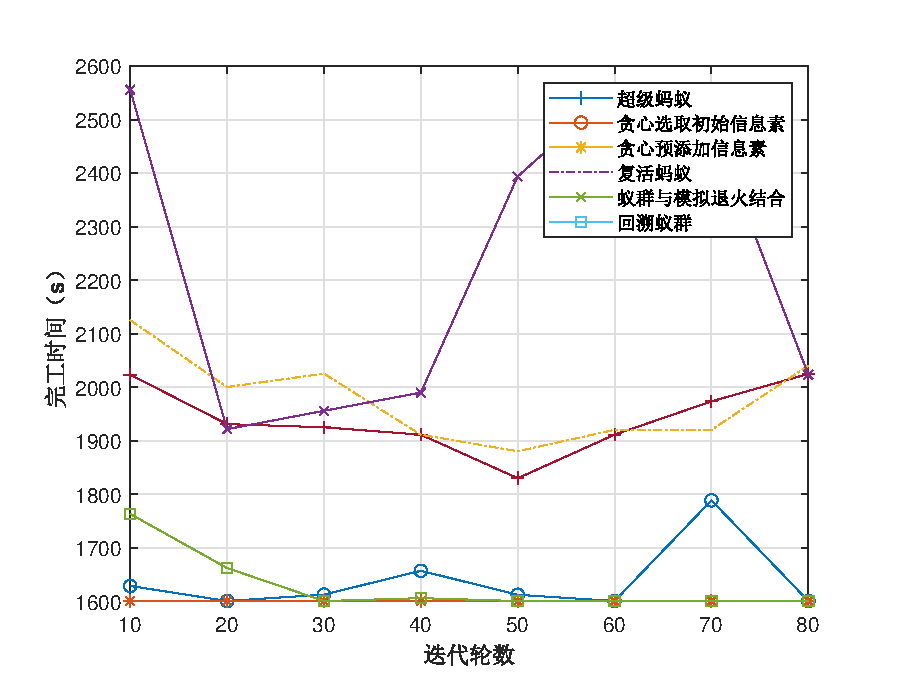
\includegraphics[scale=1.00,angle=0]{figures/test1.eps}\\
	\caption{蚁群算法各个优化思路迭代轮数与完工时间关系(10到80轮)}
\end{figure}

如上图所示,按迭代轮数与完工时间关系曲线的运动趋势可将6种优化思路分为3类:随迭代轮数增加,完工时间先递减后在较高值处振荡、完工时间始终在迪杰斯特拉解附近、随迭代轮数增加完工时间有收敛到迪杰斯特拉解的趋势。

关系曲线符合随迭代轮数增加,完工时间先递减后在较高值处振荡的优化思路有:超级蚂蚁、复活蚂蚁、蚁群与模拟退火结合

关系曲线符合完工时间始终在迪杰斯特拉解附近的优化思路有:贪心选取初始信息素、贪心预添加信息素

关系曲线符合随迭代轮数增加完工时间有收敛到迪杰斯特拉解的趋势的优化思路有:回溯蚁群

各种优化思路均对解产生了效果,单纯从解质量来看贪心选取初始信息素、贪心预添加信息素、回溯蚁群均能求解出接近迪杰斯特拉算法的解。
接下来将对各优化思路的类别进行分析。

\subsection{对随迭代轮数增加,完工时间先递减后在较高值处振荡的优化思路进行分析}
超级蚂蚁、复活蚂蚁、蚁群与模拟退火结合这三种思路随迭代轮数增加,完工时间先递减后在较高值处振荡。
将其与原始蚁群相比较,可以发现这三种优化思路都能够加快低迭代轮数时完工时间下降的速度。
复活蚂蚁机制的完工时间下降速度低于超级蚂蚁机制。
但是随着迭代轮数的继续增加,完工时间下降的趋势明显减缓,最终会在一个较高值附近振荡。
加入模拟退火机制的算法的振荡幅度显著高于其他两种机制,并且前期完工时间是从较高值快数下降的。

对于超级蚂蚁来说,如果发现更优的解,更优解会被添加上远高于其他解的信息素,前期几乎所有蚂蚁都会被引导上某条更优解。
但是基于上一节对第四章模型解分布的分析,最优解附近存在大量死锁,有走向最优解的蚂蚁很容易遇到死锁提前结束循迹。
因此即便使用超级蚂蚁,最优解上积累的信息素也会很快被其他互通的较差解超过。
算法无法收敛到最优解。

对于复活蚂蚁来说,前期完工时间下降快是因为提前结束循迹的蚂蚁被其他蚂蚁替代复活后,有效蚂蚁的数量大大增加,
实际上相当于增加了蚂蚁数量。
但是因为走向最优解并遇到死锁提前结束循迹蚂蚁会被走向较差解的蚂蚁替代,算法依然无法收敛到最优解。

对于模拟退火来说,在还未探索到较优解时,逐步提高后期蚂蚁,将避免算法局部收敛,因此算法前期波动会更大。
后期受第四章模型特殊的解分布的影响,拥有更高地位的蚂蚁反而会更剧烈地把解引导到互通的差解区域。
因此后期的解依然波动很大。

综上这三种机制并不适合求解类似第四章模型的时间Petri网。

\subsection{对完工时间始终在迪杰斯特拉解附近的优化思路进行分析}
贪心选取初始信息素、贪心预添加信息素这两种优化思路完工时间始终在迪杰斯特拉解附近。
这两种思路都和贪心的思想紧密相关。
有可能第四章模型本身适合使用贪心算法求解,因此需要排除贪心算法本身对解的影响才能分析蚁群算法效果。

使用贪心算法对第四章模型进行求解,结果如下:

变迁序列为:$t_{1}$->$t_{7}$->$t_{1}$->$t_{2}$->$t_{1}$->$t_{17}$->$t_{3}$->$t_{7}$->$t_{16}$->$t_{1}$->$t_{23}$->$t_{2}$->$t_{1}$->$t_{17}$->$t_{27}$->$t_{7}$->$t_{16}$->$t_{1}$->$t_{2}$->$t_{1}$->$t_{4}$->$t_{14}$->$t_{24}$->$t_{12}$->$t_{22}$->$t_{1}$->$t_{13}$->$t_{29}$->$t_{11}$->$t_{22}$->$t_{1}$->$t_{14}$->$t_{12}$->$t_{22}$->$t_{20}$->$t_{18}$->$t_{1}$->$t_{4}$->$t_{14}$->$t_{24}$->$t_{12}$->$t_{22}$->$t_{20}$->$t_{18}$->$t_{13}$->$t_{1}$->$t_{29}$->$t_{11}$->$t_{22}$->$t_{20}$->$t_{18}$->$t_{14}$->$t_{1}$->$t_{12}$->$t_{22}$->$t_{20}$->$t_{18}$->$t_{1}$->$t_{4}$->$t_{14}$->$t_{24}$->$t_{12}$->$t_{22}$->$t_{20}$->$t_{18}$->$t_{13}$->$t_{20}$->$t_{18}$->$t_{8}$->$t_{29}$->$t_{22}$->$t_{14}$->$t_{20}$->$t_{18}$->$t_{9}$->$t_{22}$->$t_{20}$->$t_{18}$->$t_{20}$->$t_{18}$->$t_{4}$->$t_{10}$->$t_{9}$->$t_{24}$->$t_{22}$->$t_{6}$->$t_{8}$->$t_{22}$->$t_{28}$->$t_{10}$->$t_{20}$->$t_{18}$->$t_{9}$->$t_{22}$->$t_{20}$->$t_{18}$->$t_{20}$->$t_{18}$->$t_{4}$->$t_{10}$->$t_{9}$->$t_{22}$->$t_{20}$->$t_{18}$

完工时间为:1600.8s

程序运行时间为:0.065s

变迁序列和完工时间均与迪杰斯特拉解一样,因此此网的贪心解就是最优解。

原模型为S3PR模型,本就适合最早加工策略的调度,因此使用贪心算法就能求出最优解。
破坏原模型的顺序结构,使其加工腔的晶圆可以重入得到网1 。

基于上文的分析,算法收敛到差解的主要原因是此模型存在死锁,因此需要研究算法在无死锁模型下的情况。
网1存在大量死锁,对网1进行死锁控制形成网2 。
对网1、网2使用100只蚂蚁的蚁群算法分别从10轮每次递增10轮直到80轮进行测试两种优化思路,观察完工时间。

网1的测试结果如下:

\begin{table}[H]
	\centering
	\caption{网1各优化思路完工时间与迭代轮数关系}
	\resizebox{!}{!}{
		\begin{tabular}{c|cccccccccc}
			\toprule
			\diagbox{优化思路}{完工时间(s)}{迭代轮数} & 10 & 20 & 30 & 40 & 50 & 60 & 70 & 80  \\
			\hline
			贪心选取初始信息素 & 2554.7 & 2124.5 & 2024.1 & 1973.7 & 1921.1 & 1973.7 & 1990.0 & 1973.7  \\
			贪心预添加信息素 & 2393.8 & 2024.5 & 2024.5 & 2024.1 & 1973.7 & 1920.7 & 1973.1 & 1921.1  \\
			\bottomrule
		\end{tabular}
	}
\end{table}

网2的测试结果如下:

\begin{table}[H]
	\centering
	\caption{网2各优化思路完工时间与迭代轮数关系}
	\resizebox{\linewidth}{!}{
		\begin{tabular}{c|cccccccccc}
			\toprule
			\diagbox{优化思路}{完工时间(s)}{迭代轮数} & 10 & 20 & 30 & 40 & 50 & 60 & 70 & 80  \\
			\hline
			贪心选取初始信息素 & 2040.5 & 2034.5 & 1911.5 & 1820.3 & 1788.9 & 1763.5 & 1662.4 & 1600.8  \\
			贪心预添加信息素 & 2554.7 & 2120.1 & 1973.7 & 1900.5 & 1820.3 & 1788.9 & 1700.5 & 1606.2  \\
			\bottomrule
		\end{tabular}
	}
\end{table}

\begin{figure}[H]
	\centering
	% Requires \usepackage{graphicx}
	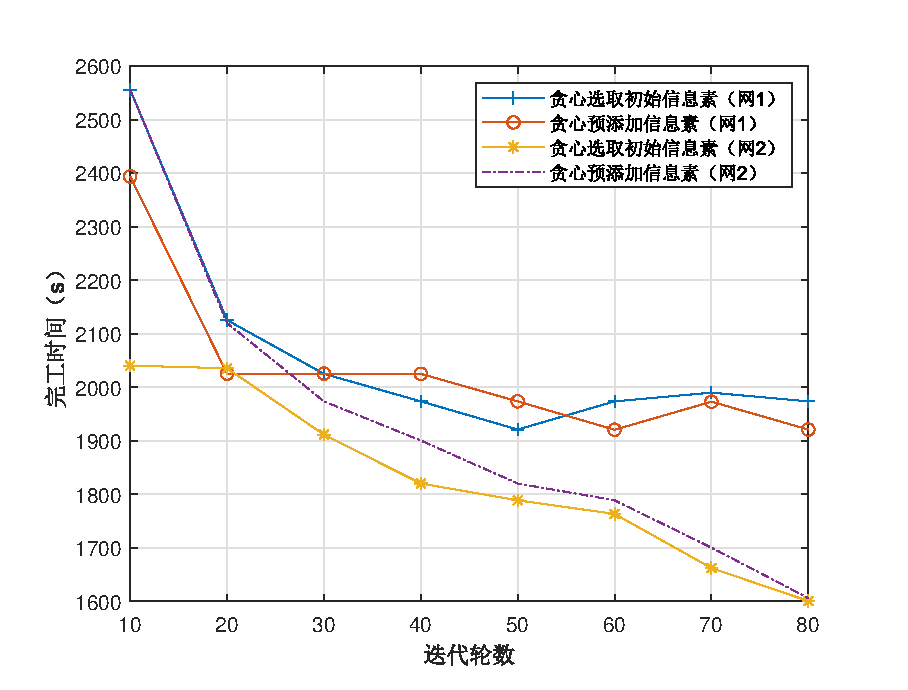
\includegraphics[scale=1.00,angle=0]{figures/test2.eps}\\
	\caption{贪心优化思路迭代轮数与完工时间关系(10到80轮)}
\end{figure}

如上图所示,如果不做死锁控制,加入贪心机制的蚁群算法依然无法收敛到最优解。
因此对于最优解附近有大量死锁的时间Petri网,这两种优化思路效果有限。但是如果在使用蚁群求解前,预先消除Petri网死锁,算法将会有很好的收敛效果。

\subsection{对随迭代轮数增加完工时间有收敛到迪杰斯特拉解的趋势的优化思路进行分析}
只有回溯蚁群机制一种优化思路能让算法随迭代轮数增加完工时间有收敛到迪杰斯特拉解的趋势。

本次测试回溯蚁群时蚂蚁寿命上限是使用统计平均寿命的方法实现的。
对静态蚂蚁寿命和最小蚂蚁寿命也在相同条件下进行实验,静态蚂蚁寿命设置为100 。

\begin{table}[H]
	\centering
	\caption{各寿命上限机制与完工时间与迭代轮数关系}
	\resizebox{!}{!}{
		\begin{tabular}{c|cccccccccc}
			\toprule
			\diagbox{蚂蚁寿命上限机制}{完工时间(s)}{迭代轮数} & 10 & 20 & 30 & 40 & 50 & 60 & 70 & 80  \\
			\hline
			静态蚂蚁寿命 & 2359.2 & 2120.1 & 1983.1 & 1900.5 & 1880.4 & 1780.5 & 1730.5 & 1616.2  \\
			最小蚂蚁寿命 & 2492.3 & 2020.4 & 2123.1 & 2124.7 & 2374.2 & 2522.5 & 2473.3 & 2554.7  \\
			\bottomrule
		\end{tabular}
	}
\end{table}

\begin{figure}[H]
	\centering
	% Requires \usepackage{graphicx}
	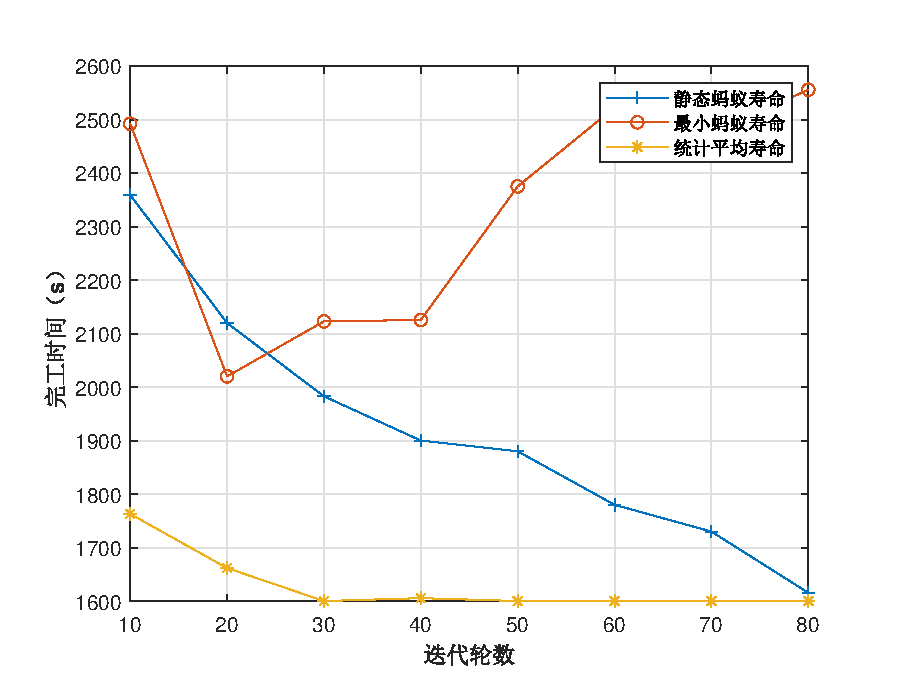
\includegraphics[scale=1.00,angle=0]{figures/test3.eps}\\
	\caption{不同蚂蚁寿命上限机制与完工时间关系(10到80轮)}
\end{figure}

如上图所示,静态蚂蚁寿命与统计平均寿命能够使算法收敛到最优解,但是最小蚂蚁寿命机制随着迭代轮数的增加,解的质量会恶化。

其原因可能是使用最小蚂蚁寿命机制时,算法后期的蚂蚁寿命上限过低,以至于蚂蚁失去回溯能力,无法走上死锁过多的路径。

统计使用最小蚂蚁寿命机制与统计平均寿命时,蚂蚁寿命上限与迭代轮数的关系。

\begin{table}[H]
	\centering
	\caption{各寿命上限机制与寿命上限与迭代轮数关系}
	\resizebox{!}{!}{
		\begin{tabular}{c|cccccccccc}
			\toprule
			\diagbox{寿命机制}{寿命上限}{迭代轮数} & 10 & 20 & 30 & 40 & 50 & 60 & 70 & 80  \\
			\hline
			静态蚂蚁寿命 & 83 & 24 & 10 & 1 & 1 & 1 & 1 & 1  \\
			统计平均寿命 & 167 & 201 & 123 & 25 & 12 & 15 & 10 & 13  \\
			\bottomrule
		\end{tabular}
	}
\end{table}

\begin{figure}[H]
	\centering
	% Requires \usepackage{graphicx}
	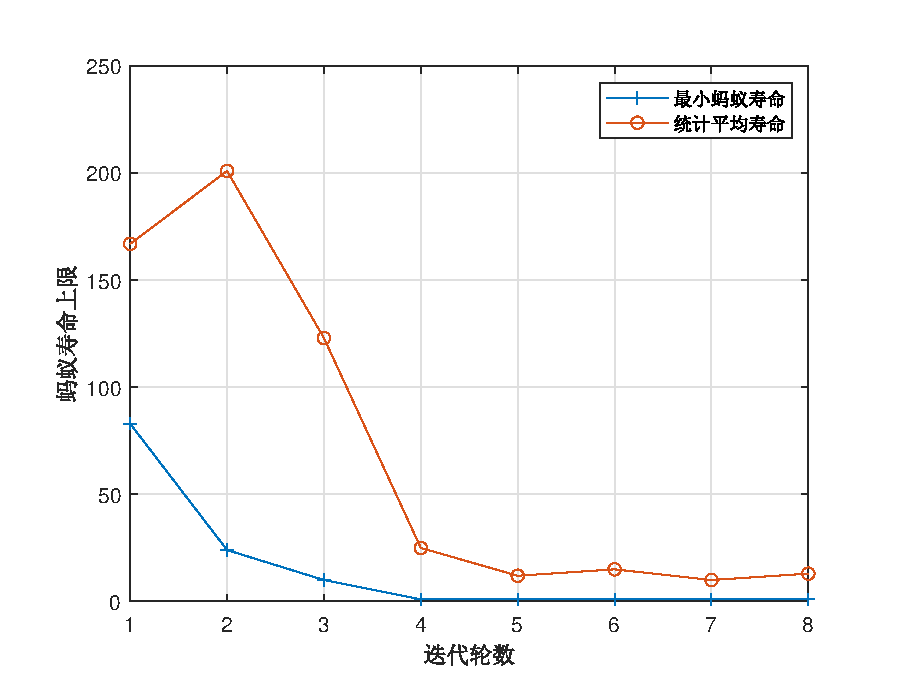
\includegraphics[scale=1.00,angle=0]{figures/test4.eps}\\
	\caption{不同蚂蚁寿命上限机制蚂蚁寿命上限与迭代轮数的关系(10到80轮)}
\end{figure}

如上图所示,使用最小蚂蚁寿命时,蚂蚁寿命上限很快降低到最小值,以至于后期蚂蚁几乎没有回溯能力。
但使用统计平均寿命时蚂蚁寿命上限最终收敛于12左右,依然具备一定的回溯能力,并且远小于直接配置静态寿命100,大大节约了程序运行时间。

\subsection{CPU数量对回溯蚁群算法速度的影响}
基于本章第1节对本蚁群算法流程的描述,本文所使用的蚁群算法为多线程算法。
所有蚂蚁均可并行地探索可达图,蚂蚁数量越多,在CPU数量不做限制时,算法将寻找到更多的解。
因此不论从解质量还是程序运行时间的角度看蚂蚁数量越多越好。

但是根据4.4.3.2节的实验数据,当蚂蚁数量在10以上时,再增加蚂蚁数量对解贡献就不大了。
而实际情况下CPU数量是有限的,线程切换时会有额外的CPU资源的开销,因此不宜设置过高的蚂蚁数量。

迪杰斯特拉算法是单线程算法,不会受到CPU数量影响,因此提升CPU数量无法减小程序运行时间。
在使用了m1 ultra的Mac Studio上使用迪杰斯特拉算法计算第四章建立的时间Petri网模型,程序运行时间为7.232s。
以此为基准,使用100只蚂蚁的蚁群算法迭代100轮,统计不同CPU数量下程序运行时间。

\begin{table}[H]
	\centering
	\caption{各寿命上限机制与寿命上限与迭代轮数关系}
	\resizebox{\linewidth}{!}{
		\begin{tabular}{c|cccccccccccc}
			\toprule
			CPU数量 & 11 & 12 & 13 & 14 & 15 & 16 & 17 & 18 & 19 & 20 \\ \hline
			程序运行时间(s) & 23.525 & 14.312 & 8.753 & 6.624 & 4.231 & 4.441 & 3.001 & 2.121 & 1.361 & 1.214 \\
			\bottomrule
		\end{tabular}
	}
\end{table}

\begin{figure}[H]
	\centering
	% Requires \usepackage{graphicx}
	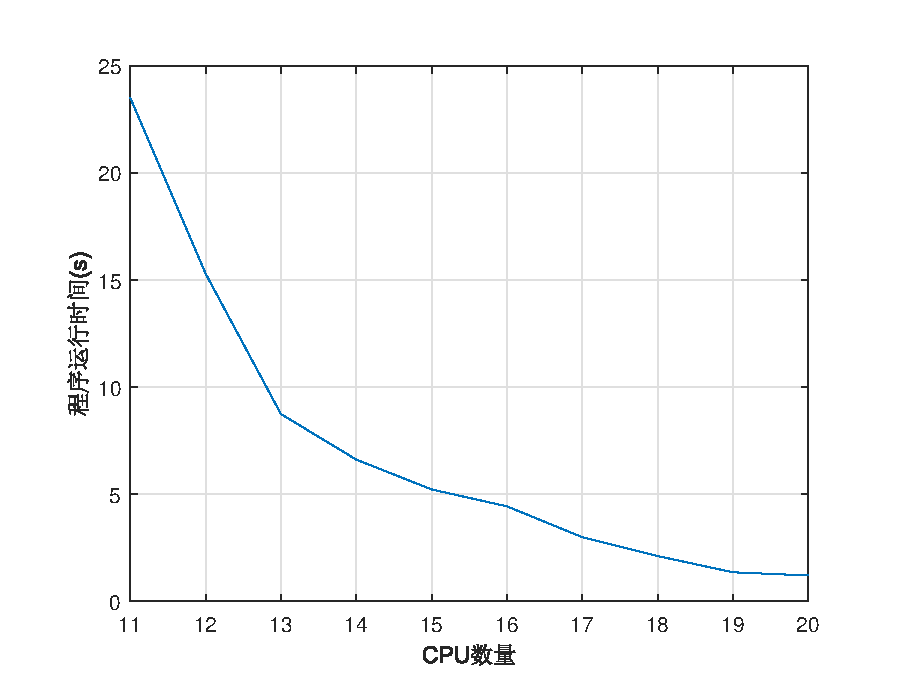
\includegraphics[scale=1.00,angle=0]{figures/test5.eps}\\
	\caption{蚁群算法不同CPU数量下程序运行时间}
\end{figure}

如上图所示,当开启14个CPU时,程序运行时间就已经优于迪杰斯特拉算法了,继续增加CPU数量能显著提升算法效果。

\section{本章小结}
本章提出了一种基于时间Petri网的蚁群算法,使用此算法求解上一章模型的调度策略,并与迪杰斯特拉算法相比较。
发现蚁群算法的解明显劣于迪杰斯特拉算法,
而且随迭代轮数增加,算法不能收敛。
于是基于实际情况,设计了6种优化方案,最终回溯蚁群策略效果明显。